\section*{Задача}
Реализовать программу, моделирующую выполнение протокола голосования для
12 файловых серверов при помощи пересылок MPI типа точка-точка. Получить
временную оценку времени выполнения одним процессом 3-х операций записи и
10 операций чтения $N$ байтов информации с файлом, расположенным (размноженным)
на 12 серверах. Определить оптимальные значения кворума чтения и кворума записи
для $N=300$. Время старта равно 100, время передачи байта равно 1
($Ts=100$,$Tb=1$).


\section*{Реализация}

Реализуем алгорим работы файловых серверов при помощи пересылок MPI типа
точка-точка. Это потребует небольшой модификации алгоритма, описанного на
лекциях и в книге Э.С.\,Таненбаума "Распределенные системы"\,, для корректной
обработке дедлоков без назначения тайм-аута, используя только передачи типа
точка-точка.

На рис. \ref{fig:all} приведена подробная блок-схема модифицированного
алгоритма. Подпрограмма "Получить все ответы"\, приведена на рис.
\ref{fig:get_all_req}.

Части схемы в большем масштабе приведены на рис. \ref{fig:read},
\ref{fig:write}, \ref{fig:idle}.

\begin{figure}[H]
    \centering
    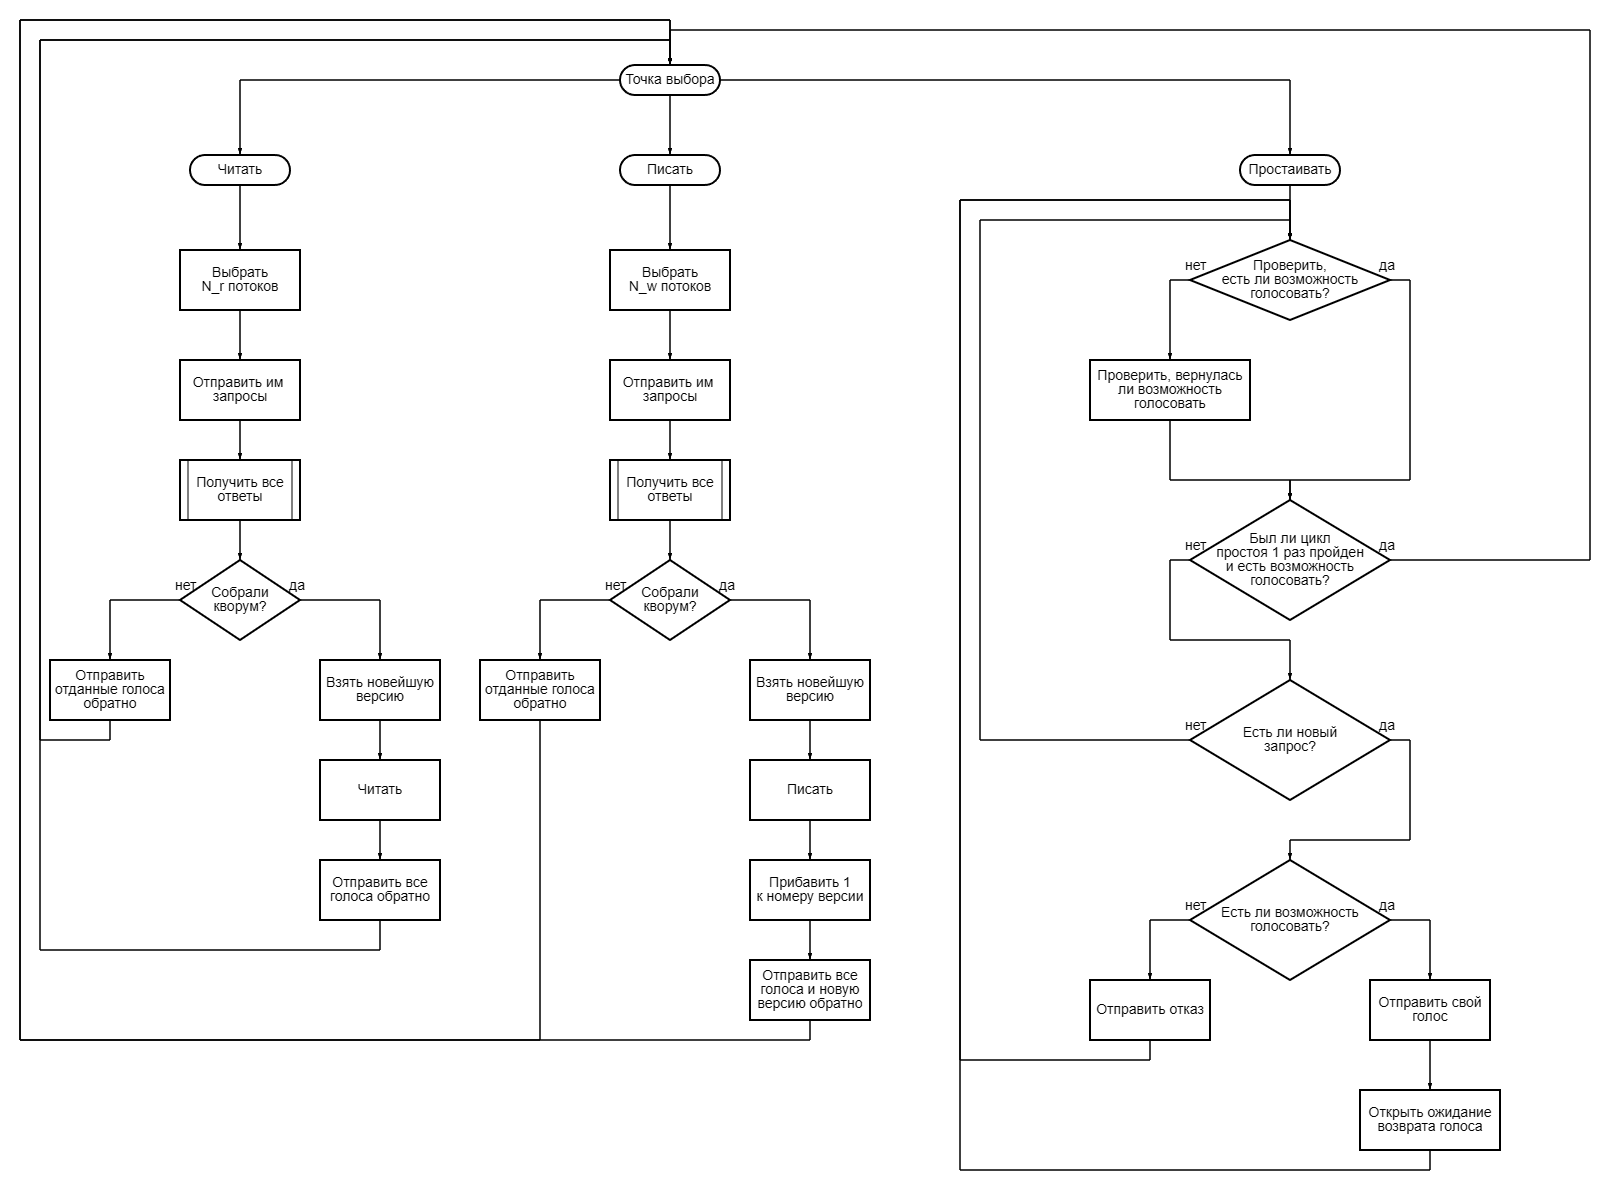
\includegraphics[width=1.\linewidth,center]{all.png}
    \caption{Схема работы алгоритма}
    \label{fig:all}
\end{figure}

\begin{figure}[H]
    \centering
    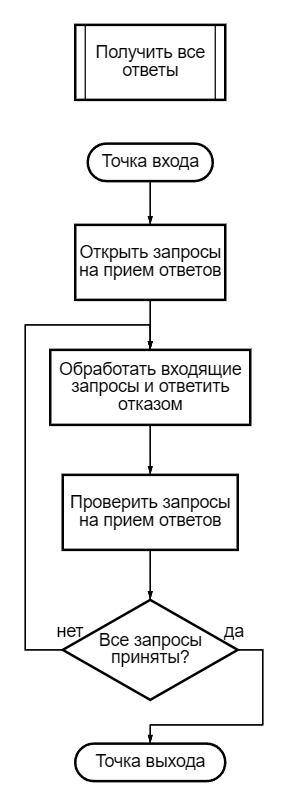
\includegraphics[width=.4\linewidth,center]{get_all_req.png}
    \caption{Подпрограмма "Получить все ответы"\,}
    \label{fig:get_all_req}
\end{figure}

Части схемы с рис. \ref{fig:all} в большем масштабе:

\begin{figure}[H]
    \centering
    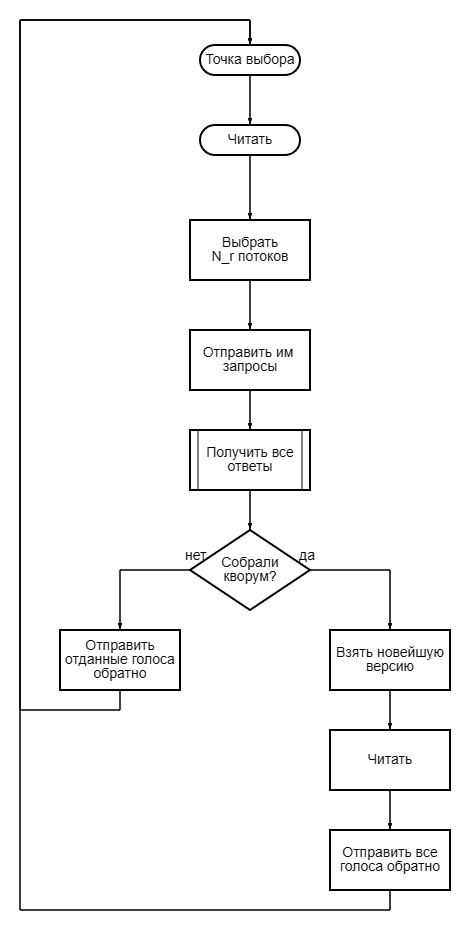
\includegraphics[width=.7\linewidth,center]{read.png}
    \caption{Схема чтения}
    \label{fig:read}
\end{figure}

\begin{figure}[H]
    \centering
    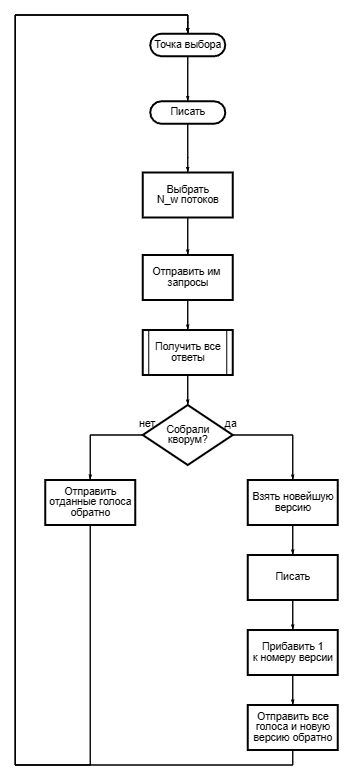
\includegraphics[width=.6\linewidth,center]{write.png}
    \caption{Схема записи}
    \label{fig:write}
\end{figure}

\begin{figure}[H]
    \centering
    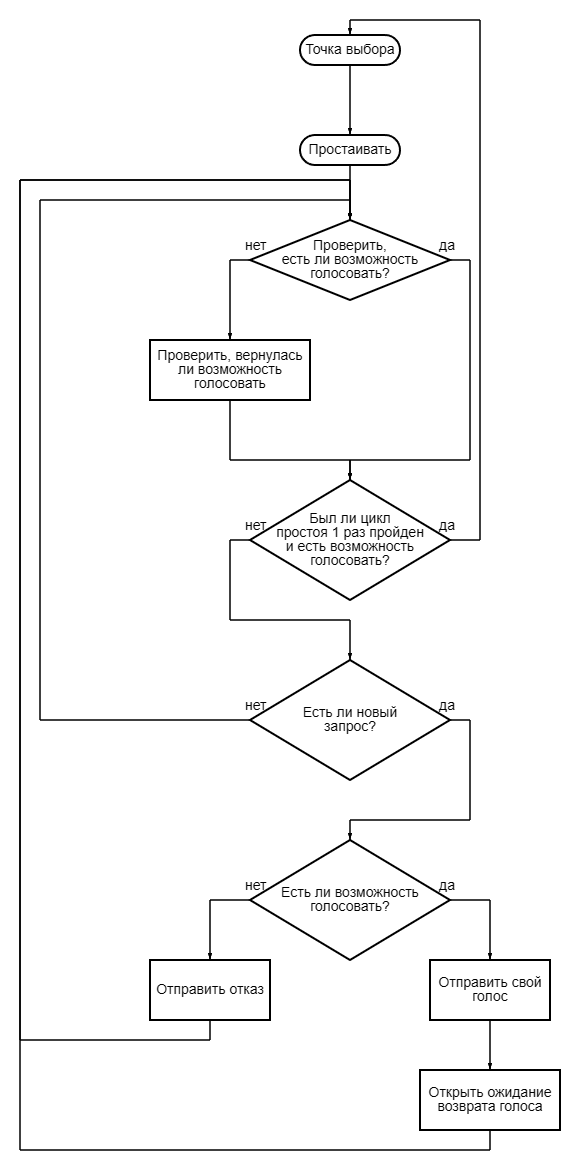
\includegraphics[width=.7\linewidth,center]{idle.png}
    \caption{Схема простаивания}
    \label{fig:idle}
\end{figure}


\section*{Теоретическая оценка алгоритма}

\subsection*{Условие:}

Получить временную оценку времени выполнения одним процессом $W = 3$ операций
записи и $R = 10$ операций чтения $M$ байтов информации с файлом, расположенным
(размноженным) на $N = 12$ серверах. Определить оптимальные значения кворума чтения
и кворума записи для $M = 300$. Время старта равно $T_s = 100$, время передачи
байта равно $T_b = 1$.

\subsection*{Решение:}

\begin{itemize}
    \item Обозначим время чтения 1 байта информации, как $T_r$, а время
        записи -- $T_w$.
    \item Обозначим кворум чтения, как $N_r$, а кворум записи -- $N_w$.
        Естественно, что $N_r + N_w > N$ и $N_w > N / 2$.
    \item Будем считать, что для запроса на чтение/запись и отправки
        согласия/отказа в ответ на такой запрос хватает 1 байта. И такие
        запросы сервер посылает и принимает последовательно,
        т.к. тип пересылок точка-точка.
\end{itemize}

1. \textit{Оценка снизу.}

Пусть $W$ операции записи и $R$ операций чтения
происходят на одном сервере и являются единственными операциями, которые
происходят за рассматриваемый промежуток времени. Таким образом передача
файла текущему серверу происходить не будет, т.к. текущий сервер всегда имеет
самую актуальную версию.

Оценим операцию чтения, как время необходимое на запрос на $N_r$ серверов,
ответ от них и отправку подтверждения, что они снова могут голосовать.
$$
3*(N_r * 1 * T_b) = 3N_rT_b
$$

Оценим операцию записи, как время необходимое на запрос на $N_w$ серверов,
ответ от них, отправку подтверждения, что они снова могут голосовать и новой
версии файла.
$$
3*(N_w * 1 * T_b) + N_w*M*T_b = N_wT_b(3 + M)
$$

Итоговая оценка снизу:
$$
T_s + 3N_rT_bR + N_wT_b(3 + M)W = 100 + 30N_r + 909N_w
$$

2. \textit{Оценка сверху.}

Пусть $W$ операции записи и $R$ операций чтения происходят на одном сервере, но
каждый раз между ними происходит запись в файл и обновление его версии,
инициированное сторонним сервером.

Для простоты будем считать, что сторонний сервер не обращается к нашему
серверу, т.к. тогда расходы на передачу версии файла могут неограниченно расти,
если предположить, что таких записей от сторонних серверов может быть
бесконечно много.

Оценим операцию чтения, как время необходимое на запрос на $N_r$ серверов,
ответ от них, запрос на получение самой новой версии файла, получение файла и
отправку подтверждения серверам, что они снова могут голосовать.
$$
N_r*1*T_b + N_r*1*T_b + 1*T_b + M*T_b + N_r*1*T_b = (3N_r + 1 + M)T_b
$$

Оценим операцию записи, как время необходимое на запрос на $N_w$ серверов,
ответ от них, запрос на получение самой новой версии файла, получение файла и
отправку подтверждения, что они снова могут голосовать и новой версии файла.
$$
N_w*1*T_b + N_w*1*T_b + 1*T_b + M*T_b + N_w*1*T_b + N_w*M*T_b = (3N_w + N_wM + 1 + M)T_b
$$

Итоговая оценка сверху:
$$
T_s + (3N_r + 1 + M)T_bR + (3N_w + N_wM + 1 + M)T_bW = 4013 + 30N_r + 909N_w
$$

3. \textit{Определение оптимального значения кворумов чтения и записи.}

В п.1 и п.2 была получена оценка времени выполнения указанных операций чтения и
записи:
$$
100 + 30N_r + 909N_w \le T \le 4013 + 30N_r + 909N_w
$$

Таким образом имеем

$$
\begin{cases}
    \min (30N_r + 909N_w)\\
    N_r + N_w > N\\
    N_w > N / 2
\end{cases}
$$



% \section{Ход работы}

% \textit{Ниже написан полнейший БРЕД (точнее компиляция лабораторных), чтобы показать, как делать то или иное действие в латехе и оверлифе. Все совпадения случайны.}

% Дана система с произвольной задержкой

% $\dot{x} = Ax(t) + A_1 x (t-h), $
% $A =
% \begin{bmatrix}
% 1 &  0\\
% 4 & 3\\
% \end{bmatrix},
% A_1 =
% \begin{bmatrix}
% -2 & 1 \\
% -2 & -6\\
% \end{bmatrix}$

% $\begin{bmatrix}
% \Phi & P - P_2^T (A+A_1)^T P_3 & -h P_2^T A_1\\
% * & -P_3 - P_3^T + hR & -h P_3^T A_1\\
% * & * & -hR\\
% \end{bmatrix} < 0,
% $

% $\Phi = P_2^T (A+A_1) + (A+A_1)^T P_2, P > 0, R > 0$

% Здесь $P_2$ и $P_3$ – произвольные матрицы. В результате решения матричного неравенства выше в MATLAB получена максимальная задержка $h = 0.18$, при которой система является устойчивой.

% Схема моделирования была собрана. Опытным путём удалось установить значение $K_{OC} = 2.5$ - максимальное допустимое, то есть значение при котором система устойчива (это граница устойчивости).

% \begin{figure}[H]
%     \centering
% \includegraphics[width=1.\linewidth,center]{scheme_1.png}
%     \caption{Схема моделирования}
%     \label{fig:my_label}
% \end{figure}

% % место для вывода про экстраполятор

% \subsection{Что-то там про колебательность}

% Колебательность процесса при фиксированном периоде квантования $T$ зависит от $K_{OC}$ следующим образом: чем больше $K_{OC}$ - тем больше система будет колебаться, пока не дойдёт до границы устойчивости, на которой она будет вести себя как чисто колебательная система без стремления к нулю.

% На графиках ниже можно видеть, как переходный процесс становится всё более колебательным и колебательным.

% Пусть степень устойчивости $\alpha = 0.5$. Тогда

% \begin{enumerate}
%     \item При $\mu = 3, \; \sigma(A+BK) = \{  -1.3192 \pm 5.2207i,  -0.9915, -1\}$
%     \item При $\mu = 1, \; \sigma(A+BK) = \{  -1.1340 \pm 5.5547i,  -0.9361, -1\}$
%     \item При $\mu = 0.4, \; \sigma(A+BK) = \{  -0.9402 \pm 5.8582i,  -0.7433, -1\}$
% \end{enumerate}


% \subsubsection{Графики}

% \begin{figure}[H]
%     \centering
% \includegraphics[width=1.\linewidth,center]{plot_y_2.png}
%     \caption{График $y(t)$ при $K_{OC} = 2$}
%     \label{fig:my_label}
% \end{figure}


% \begin{figure}[H]
%     \centering
% \includegraphics[width=1.\linewidth,center]{plot_y_23.png}
%     \caption{График $y(t)$ при $K_{OC} = 2.3$}
%     \label{fig:my_label}
% \end{figure}


% \begin{figure}[H]
%     \centering
% \includegraphics[width=1.\linewidth,center]{plot_y_25.png}
%     \caption{График $y(t)$ при $K_{OC} = 2.5$}
%     \label{fig:my_label}
% \end{figure}

% \begin{figure}[!htbp]
% \centering
% \begin{subfigure}{.5\textwidth}
%   \centering
%   \includegraphics[width=0.8\linewidth]{download (16).png}
%   \caption{Зелёные}
%   \label{fig:sub1}
% \end{subfigure}%
% \begin{subfigure}{.5\textwidth}
%   \centering
%   \includegraphics[width=0.8\linewidth]{download (17).png}
%   \caption{Оранжевые}
%   \label{fig:sub2}
% \end{subfigure}
% \label{fig:test}
% \caption{Сегментированные области}
% \end{figure}

% Максимальная колебательность наблюдается при $K_{OC} = 2.5$

% \subsubsection{Код Python}

% \begin{lstlisting}[language=Python, caption=Импорт и обычная бинаризация]
% import cv2
% from google.colab.patches import cv2_imshow
% from matplotlib import pyplot as plt
% import numpy as np
% from math import *
% import skimage
% from skimage import data, io, filters

% I=cv2.imread("pic.jpg",cv2.IMREAD_GRAYSCALE)
% cv2_imshow(I)
% t=127
% ret,Inew=cv2.threshold(I,t,255,cv2.THRESH_BINARY)
% plt.imshow(Inew)
% \end{lstlisting}
